\section{Voice at 250 Bits per Second}
\label{sec:cport_voice}

Every payload so far has been data.  Voice was never plausible on this
link: the classic amateur speech codecs start around 700\,bit/s
(Codec2 700C, what FreeDV uses on HF), and rung~12 carries a measured
102\,B/s $=$ 816\,bit/s of \emph{goodput}, leaving no room for framing,
acknowledgements or a fade.  Neural codecs have since moved the floor.
LSCodec-25\,Hz~\cite{guo2025lscodec} (MIT licensed)
emits 25 tokens per second, each a 10-bit index into a 1024-entry
codebook: \textbf{250\,bit/s}, or 31.25\,B/s.  That is a quarter of
what the top rung carries.

This section has three parts.  The first (\S\ref{sec:voice_eval},
\S\ref{sec:voice_streaming}) is evaluation: the measurements decide
what a voice mode costs and which of its problems are fixable, all of
it host-side, codec in and codec out.  The second
(\S\ref{sec:voice_onair}) is the mode as built: the codec on the air
between the two boards --- push a button, speak, and the far station
writes a \texttt{.wav} --- and the firmware changes that exercise
required, none of which a host-side measurement could have predicted.
The third (\S\ref{sec:voice_loss}) is the group loss that the clean
wire kept reporting, the two wrong explanations that survived their own
measurements, and the receiver defect that was the cause.

\subsection{The link is not the constraint}

At 31.25\,B/s one station message (\texttt{ST\_MSG\_MAX} 3328) holds
\textbf{106 seconds of speech}, and the streaming burst machinery
already carries it: a 200-byte fragment is exactly 160 tokens, or
6.4\,s.  Table~\ref{tab:voice_rate} gives the delivery ratio against
the ladder.

\begin{table}[H]
    \centering
    \caption{Speech delivered per second of air, from the streamed
             goodput of each rung (the ladder's raw rate less the
             per-frame overhead; the rung-12 figure is the 130\,B/s a
             stream carries, against the 102--114\,B/s an
             acknowledged file transfer nets end to end,
             \S\ref{sec:cport_levers}).  Real time is the $1.00\times$
             line;
             the modem's headline sensitivity, EXTREME at
             $-17.9$\,dB, is unusable for voice by three orders of
             magnitude.}
    \label{tab:voice_rate}
    \small
    \begin{tabular}{@{}lrrrr@{}}
    \toprule
    \textbf{Rung} & \textbf{Sens.\ (dB)} & \textbf{Goodput} &
    \textbf{106\,s memo} & \textbf{Speech/s of air} \\
    \midrule
    0 (EXTREME)  & $-17.9$ &   1.0\,B/s & 3465\,s & $0.03\times$ \\
    4 (NORMAL)   & $-7.6$  &  14.5\,B/s &  230\,s & $0.46\times$ \\
    7            & $-5.3$  &  43.5\,B/s &   77\,s & $1.39\times$ \\
    10           & $+0.7$  &  86.9\,B/s &   38\,s & $2.78\times$ \\
    \textbf{12}  & $+4.7$  & \textbf{130\,B/s} & \textbf{26\,s} &
    $\mathbf{4.17\times}$ \\
    \bottomrule
    \end{tabular}
\end{table}

Voice runs faster than real time from rung~7 upward and is
store-and-forward below it.  The cost is that the link's whole
sensitivity advantage is forfeited: at the EXTREME bootstrap rung a
106-second memo needs an hour of air.  A voice mode is a
good-conditions mode.

Compute is likewise not the constraint, provided it stays on the host.
Measured on the demonstration laptop (Intel i5-8300H, CPU only), the
17.5\,M-parameter encoder runs at $14.3\times$ real time on
\emph{one} core and $31\times$ on four; the 31.3\,M-parameter vocoder
decodes at roughly $3\times$.  Encoding a 106-second memo takes
3.4--7.4\,s against 26\,s of air, so it overlaps keying.  Memory is the
awkward figure: a one-shot encode costs about 14\,MB per second of
audio, so a full-length memo peaks near 2\,GB.  None of this belongs on
the STM32 --- 48\,M parameters of PyTorch is four orders of magnitude
beyond the part --- which places a voice mode exactly where KISS
(\S\ref{sec:cport_kiss}) and the IP tunnel (\S\ref{sec:cport_iptun})
already are: a host program above an unchanged modem.

\subsection{Codec Evaluation}
\label{sec:voice_eval}

The measurements below are of the codec alone, with no channel between
encoder and decoder; the link enters only through the byte budget of
Table~\ref{tab:voice_rate}.

\subsubsection{Two findings that are not about the bitrate}

\paragraph{The codec is domain-sensitive, and fails abruptly.}
Reconstruction quality was measured as ASR word error rate against
ground-truth transcripts, using a CTC recogniser
(\texttt{wav2vec2-large-960h-lv60-self}) rather than an
attention-decoder model, because the latter hallucinates on damaged
audio and scores it as total loss.  The result depends on the corpus
far more than on anything in the codec.

\begin{table}[H]
    \centering
    \caption{The same weights, prompt scheme and recogniser on two
             corpora, 16 and 15 utterances.  LibriTTS is what LSCodec
             was trained on; LibriSpeech is ordinary read speech from
             the same books, recorded and processed differently.}
    \label{tab:voice_domain}
    \small
    \begin{tabular}{@{}lrrr@{}}
    \toprule
    & \textbf{LibriTTS} & \textbf{LibriSpeech} & \textbf{Paper} \\
    & \emph{(in domain)} & \emph{(out of domain)} & \emph{(reported)} \\
    \midrule
    WER, original audio      & 8.28\,\% & 1.01\,\%  & 1.20\,\% \\
    WER, after 250\,bit/s    & 10.83\,\% & 22.64\,\% & 5.46\,\% \\
    \textbf{Added by codec}  & \textbf{+2.6\,pts} & \textbf{+21.6\,pts}
                             & +4.3\,pts \\
    Speaker similarity       & 0.875 & 0.864 & 0.945 \\
    \textbf{Utterances destroyed} & \textbf{0 of 15} & \textbf{3 of 16}
                             & --- \\
    \bottomrule
    \end{tabular}
\end{table}

On its own corpus the codec costs 2.6 points of word error and loses
nothing outright, reproducing the paper's 4.3.  Move one corpus away
and it costs 21.6 points and destroys three utterances in sixteen ---
not degraded, destroyed: normal duration, normal energy, and a
transcript reading \texttt{Eatly Waty Ing Ening} where the sentence
was ``it is obviously unnecessary for us to point out\ldots''.  The
same failures appear under a second recogniser of a different
architecture, so this is the audio and not a transcription artefact.

That failure mode is the important one for a radio link, because it is
\textbf{invisible to every layer below the ear}.  The bitstream is
valid, the CRC passes, the ARQ is satisfied, the byte count is right,
and the far operator hears confident nonsense.  Shack audio --- a real
microphone, a real room, SSB processing --- sits further from LibriTTS
than LibriSpeech does, so the right planning figure is the middle
column, not the paper's.

Four candidate explanations were tested and eliminated before the
corpus one was accepted: a substituted prompt encoder (the official
WavLM checkpoint's distribution link returns
\texttt{AuthenticationFailed}; using the authentic weights improved
speaker similarity 0.793\,$\rightarrow$\,0.845 but moved word error not
at all), a weak recogniser, a poor prompt choice (giving each utterance
\emph{itself} as prompt changed nothing), and a feature-layer indexing
error.  The pipeline reproduces the paper on the paper's own corpus,
which is what licenses the comparison.

\paragraph{The prompt, not the bitstream, carries the speaker.}
LSCodec is speaker-\emph{decoupled} by design --- that is how it
reaches 250\,bit/s.  The tokens carry what was said; a reference prompt
supplies who says it.  Decoding one byte-identical token stream against
two different prompts gives two different people:

\begin{table}[H]
    \centering
    \caption{Speaker-embedding cosine similarity (Resemblyzer).  The
             token stream is identical across each speaker's rows; only
             the prompt differs.}
    \label{tab:voice_identity}
    \small
    \begin{tabular}{@{}lrrl@{}}
    \toprule
    \textbf{Reconstruction} & \textbf{vs A} & \textbf{vs B} &
    \textbf{Outcome} \\
    \midrule
    A, matched prompt & 0.845 & 0.429 & still A \\
    A, crossed prompt & 0.428 & 0.673 & \textbf{became B} \\
    B, matched prompt & 0.478 & 0.778 & still B \\
    B, crossed prompt & 0.760 & 0.570 & \textbf{became A} \\
    \midrule
    \emph{two unrelated real speakers} & 0.431 & --- & baseline \\
    \bottomrule
    \end{tabular}
\end{table}

A crossed reconstruction scores 0.428 against its own speaker, landing
on the 0.431 baseline between two unrelated people.  A wrong prompt
does not colour the voice, it substitutes a stranger's.  For amateur
service that is a station-identification question before it is an
audio-quality one, and it is architectural: no amount of retraining
makes a speaker-decoupled token carry timbre.

\subsubsection{What enrolment costs}

The prompt is not a fixed-size speaker vector but a \emph{time series}
of WavLM-Large layer-6 features, $T \times 1024$ float32 at
$\sim$50\,Hz --- 200\,kB per second of prompt audio, some
6400$\times$ the speech bitrate.  Sending features over the air is out
of the question.  Sending prompt \emph{audio} is not, because the
quality saturates almost immediately.

\begin{table}[H]
    \centering
    \caption{Enrolment prompt length against reconstruction speaker
             similarity, and what each length would cost to transfer.
             Air time at the measured rung-12 goodput of 102\,B/s.}
    \label{tab:voice_prompt}
    \small
    \begin{tabular}{@{}lrrrr@{}}
    \toprule
    \textbf{Prompt} & \textbf{SECS} & \textbf{fp16 features} &
    \textbf{Opus 16\,kbit/s} & \textbf{Air} \\
    \midrule
    0.5\,s & 0.751 &  48\,kB & 1.0\,kB & 10\,s \\
    1\,s   & 0.826 &  98\,kB & 2.0\,kB & 20\,s \\
    \textbf{2\,s} & \textbf{0.855} & 198\,kB & \textbf{4.0\,kB} &
    \textbf{40\,s} \\
    4\,s   & 0.858 & 398\,kB & 8.0\,kB & 78\,s \\
    16\,s  & 0.869 & 1592\,kB & 32\,kB & 314\,s \\
    \bottomrule
    \end{tabular}
\end{table}

Two seconds buys 98\,\% of the benefit; eight times more data adds
0.014.  So enrolment is a one-off exchange of about 4\,kB --- roughly
40\,s of air, or two station messages --- after which every
transmission from that station is pure 250\,bit/s payload.  Two
constraints follow.  The prompt cannot be sent \emph{through} LSCodec,
which strips exactly the information it needs to carry, so a voice mode
needs a second, conventional codec for enrolment alone.  And each
station must hold WavLM-Large (1.2\,GB) locally to turn received
prompt audio into features; the cached result is about 198\,kB per
correspondent.

\subsubsection{How the prompt reaches the vocoder}
\label{sec:voice_arch}

The prompt is not a speaker vector but a \emph{time series}:
WavLM-Large~\cite{chen2022wavlm} layer-6 features, $T' \times 1024$ at $\sim$50\,Hz, with
$T' = \lfloor (n-400)/320 \rfloor + 1$ for $n$ input samples --- 99
frames for the 2\,s enrolment above.  Figure~\ref{fig:voice_codec_paths}
shows where it enters.

\begin{figure}[htbp]
    \centering
    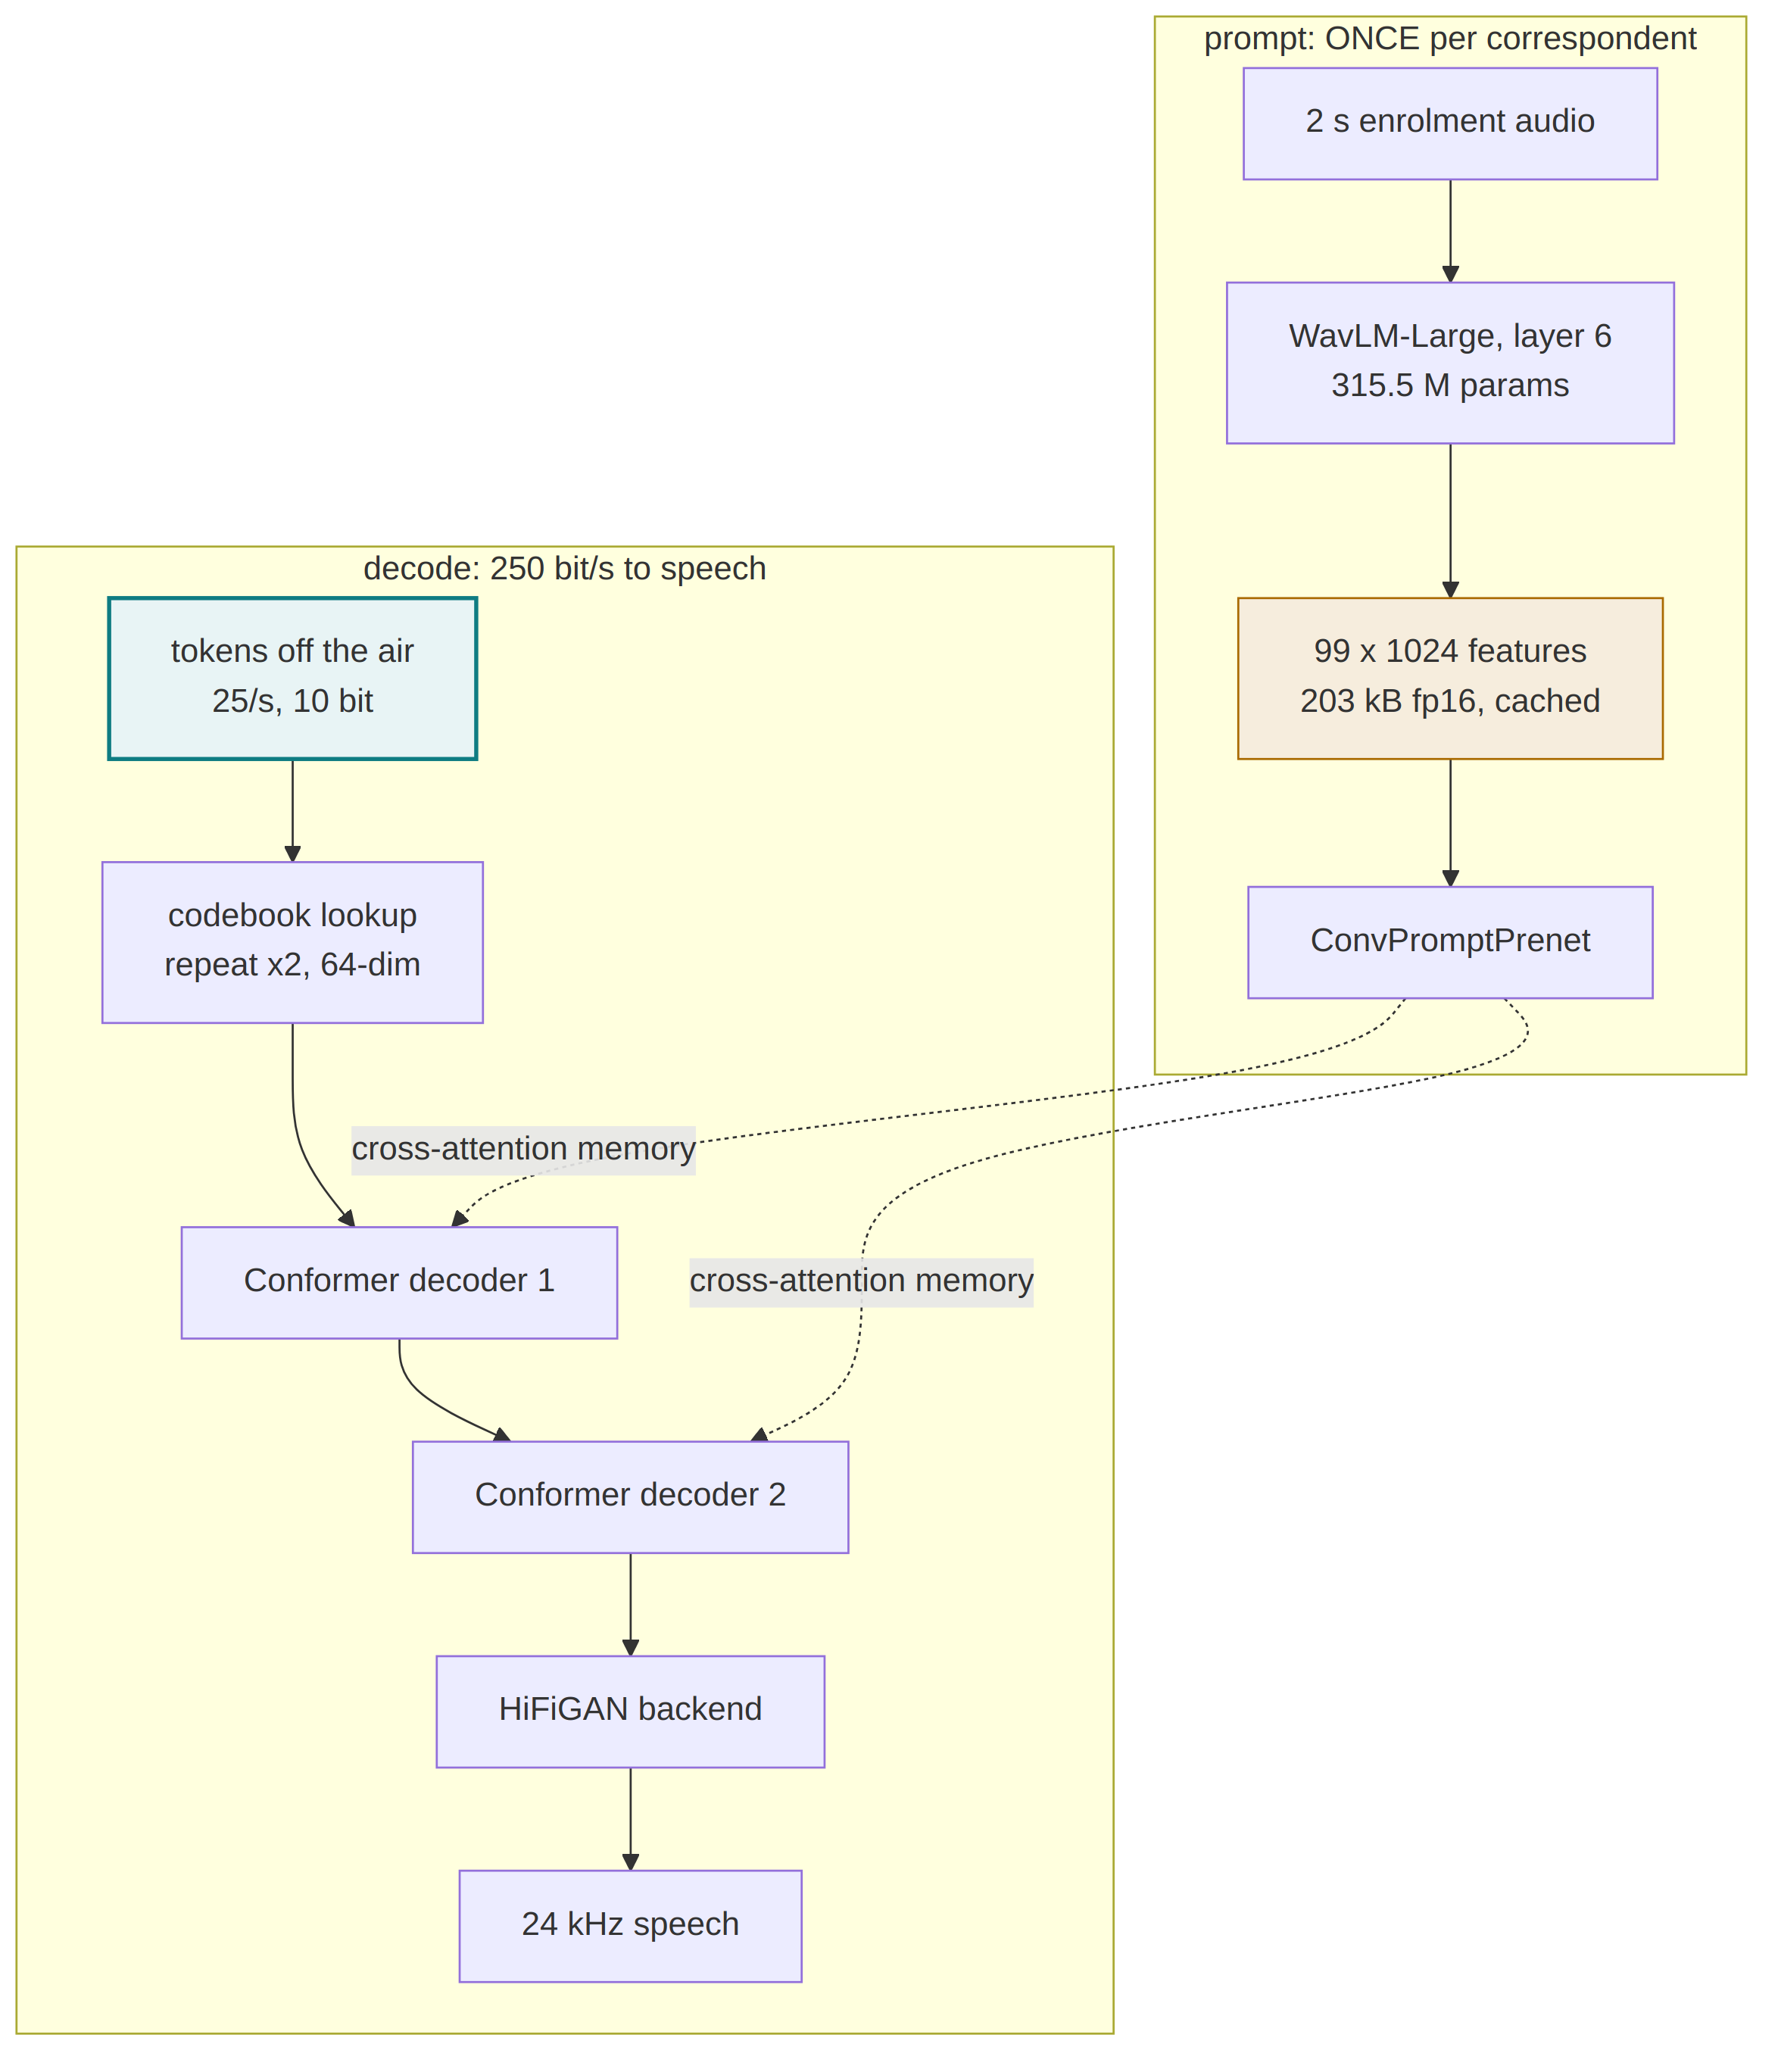
\includegraphics[width=\textwidth,height=0.80\textheight,keepaspectratio]{images/voice_codec_paths.png}
    \caption{The decode path and the prompt path.  The prompt is
             \textbf{cross-attention memory} for both Conformer stages,
             not a concatenated or pooled input --- which is why its
             length is independent of the content's, and why 99 prompt
             frames can condition a 640-frame message.}
    \label{fig:voice_codec_paths}
\end{figure}

Two details cost time to establish and are recorded here because neither
is discoverable from the configuration.  The vocoder for LSCodec-25\,Hz
was trained at 50\,Hz, so the token sequence must be
\texttt{repeat\_interleave}d by two before the codebook lookup; the only
trace of this is the \texttt{repeat\_input\_tokens} flag, and omitting it
yields speech at half speed.  And the frontend's own docstring describes
the prompt as a ``mel-spectrogram prompt'' --- inherited text from
CTX-vec2wav.  It is not mel: it is 1024-dimensional WavLM, and feeding
mel produces confident nonsense with no error raised.

\subsubsection{Can the prompt be made smaller?}
\label{sec:voice_promptsize}

At 200\,kB per second of prompt audio, the enrolment is $\sim$6400
times the speech bitrate, which is what makes it the awkward part of the
design.  Three families of compression were measured against a single
metric: mean absolute log-mel distance between the decode under a
degraded prompt and the decode under the exact one, on the same token
stream.  The scale is anchored at both ends --- 0\,dB is the correct
prompt, and \textbf{8.88\,dB is a different real speaker's prompt},
i.e.\ the point at which the speaker is simply wrong.

Pruning is ruled out by the distribution before any decode: only
3.3\,\% of values fall below 0.1 in magnitude, and \emph{zero} of the
1024 channels have low variance.  There is nothing to prune.  The
distribution is also heavily outlier-dominated --- kurtosis 52.6, range
$-35.6\ldots+57.4$ while 98\,\% of values lie within $\pm 8$, with
per-channel offsets whose median magnitude is 0.74 and maximum 47 ---
which decides how quantisation must be applied.

\begin{table}[H]
    \centering
    \caption{Prompt compression, all on the same 400-byte token stream.
             Per-channel affine quantisation is essential: at 4 bits it
             costs 0.35\,dB, while a single global scale costs 2.36\,dB
             for the same storage.}
    \label{tab:voice_quant}
    \small
    \begin{tabular}{@{}lrrl@{}}
    \toprule
    \textbf{Prompt representation} & \textbf{Bytes} & \textbf{mel dB} &
    \textbf{Verdict} \\
    \midrule
    fp32 (reference)              & 406\,kB & 0.00 & --- \\
    fp16 (as cached)              & 203\,kB & 0.00 & free \\
    \textbf{int8, per-channel}    & \textbf{105\,kB} & \textbf{0.03} &
                                    \textbf{free; use this} \\
    int6, per-channel             &  80\,kB & 0.09 & free \\
    int4, per-channel             &  55\,kB & 0.35 & small \\
    int2, per-channel             &  29\,kB & 1.50 & audible \\
    \midrule
    int8, per-tensor              & 101\,kB & 0.16 & $5\times$ worse, same size \\
    int4, per-tensor              &  51\,kB & 2.36 & ruined by outliers \\
    low-rank $k=20$               &  47\,kB & 0.89 & loses to int4 \\
    every 2nd frame               & 102\,kB & 1.31 & loses to int4 \\
    \bottomrule
    \end{tabular}
\end{table}

The interesting failure is vector quantisation, because it is the only
scheme that could plausibly beat sending audio.  A \emph{shared}
codebook --- trained once and shipped with the software, so only indices
cross the air --- was fitted on 280\,s of speech from other speakers,
with the test speaker held out.

\begin{table}[H]
    \centering
    \caption{Vector-quantising the prompt against a shared codebook.
             Every variant is at or past the point where the speaker is
             simply wrong (8.88\,dB), including the ones that would beat
             2\,s of Opus audio on size.}
    \label{tab:voice_vq}
    \small
    \begin{tabular}{@{}lrrr@{}}
    \toprule
    \textbf{Scheme} & \textbf{Bytes} & \textbf{vs 4\,kB Opus} &
    \textbf{mel dB} \\
    \midrule
    int4 per-channel (best scalar) & 54.8\,kB & $13\times$ worse & 0.35 \\
    PQ, 32 blocks $\times$ 256     &  3168\,B & about equal      & 7.87 \\
    PQ, 8 blocks $\times$ 256      &   792\,B & $5\times$ better & 9.88 \\
    full-frame VQ, $K=1024$        &   123\,B & $33\times$ better & 10.34 \\
    \midrule
    \emph{a different real speaker} & --- & --- & \emph{8.88} \\
    \bottomrule
    \end{tabular}
\end{table}

This is a rate limit, not a codebook-quality limit, and the distinction
matters because only the latter would be fixed by more training data.
The k-means converged (identical at 12 and 60 iterations) with zero dead
centroids out of 8192.  In feature space, PQ at 0.25\,bits per dimension
reaches a relative $L_2$ error of 0.593, against 0.072 for int4 at
4\,bits per dimension --- and 0.764 for simply substituting the
per-channel mean.  Three-quarters of a bit short of that baseline is not
a codebook that needs more speakers.  The features are also not
redundant enough to escape through rank: 90\,\% of the variance still
needs 40 of 99 components, and adjacent frames correlate only 0.79.

The reason is worth stating plainly, because it generalises past this
codec.  \textbf{WavLM features are an expansion of the audio, not a
compression of it}: 2\,s of speech is 32\,000 samples and 101\,376
feature values, $3.2\times$ more data.  Opus reaches 4\,kB by coding the
audio, which is a far more redundant signal.  Coding the expanded
representation instead cannot win, and the conclusion is that
\textbf{the enrolment goes over the air as audio and every station keeps
WavLM locally}.  Quantisation is a storage decision --- int8
per-channel, 105\,kB per correspondent --- not an architectural one.

A secondary observation, unexpected and useful for anyone tempted by
this: the vocoder tolerates a \emph{valid but wrong} prompt better than
a \emph{correct but corrupted} one.  Quantised prompts land off the
feature manifold and decode worse than a constant.

\subsubsection{Borrowing a purpose-built speaker encoder}
\label{sec:voice_facodec}

If the prompt cannot be compressed, the alternative is to replace it.
Several codecs represent the speaker as a small \emph{time-invariant}
code rather than a sequence: TiCodec~\cite{ren2024ticodec} splits speech
into time-dependent and time-invariant parts and quantises the latter
into eight discrete tokens per utterance; FreeCodec~\cite{zheng2024freecodec}
takes an ECAPA-TDNN speaker embedding and quantises it with group VQ,
eight groups against a 1024-entry codebook --- \textbf{80 bits, ten
bytes, for the whole utterance}; FACodec, the codec inside
NaturalSpeech~3~\cite{ju2024naturalspeech3}, factorises speech into
content, prosody, acoustic detail and timbre, extracting timbre with a
Transformer encoder.  A recent review~\cite{guo2025tokenreview} maps the
space.

Ten bytes instead of four kilobytes would remove the enrolment exchange
\emph{and} the 1.2\,GB WavLM dependency, so it is worth knowing how far
apart the representations are.  FACodec's timbre extractor was run
against LSCodec's vocoder directly: 69 utterances from 23 LibriTTS
test-clean speakers, 2\,s each, both representations computed, and a
ridge adapter fitted from the 256-dimensional timbre vector to the
1024-dimensional prompt, evaluated on speakers it never saw.

\begin{table}[H]
    \centering
    \caption{FACodec timbre driving LSCodec's vocoder.  Two losses are
             separable, and the first one bounds the whole approach.}
    \label{tab:voice_facodec}
    \small
    \begin{tabular}{@{}lr@{}}
    \toprule
    \textbf{Prompt fed to the vocoder} & \textbf{mel dB} \\
    \midrule
    true prompt, full sequence (reference)      & 0.00 \\
    \textbf{true prompt's own mean, broadcast --- the CEILING}
                                                & \textbf{3.64} \\
    FACodec timbre $\rightarrow$ ridge $\rightarrow$ broadcast & 7.18 \\
    a different real speaker, full sequence     & 8.88 \\
    corpus mean, timbre ignored (null)          & 10.16 \\
    \bottomrule
    \end{tabular}
\end{table}

The adapter carries real information --- held-out cosine $+0.36$ and
$R^2$ $+0.12$ on the speaker-discriminative component, and its decode
beats both the null and a different real speaker --- but it lands at
7.18\,dB against a ceiling of 3.64.  That ceiling is the finding.  It is
what \emph{any} time-invariant code scores with this vocoder, even given
the true prompt's own mean, because the two Conformer stages cross-attend
over 99 frames and genuinely use their temporal detail.  A constant
memory throws that away before the speaker question is even reached.

So the answer is not a better adapter, and not more speakers: the
vocoder's prompt path would have to be retrained to consume a global
code.  That is precisely what TiCodec and FreeCodec do from scratch, and
why eight tokens suffice for them.  The adapter figure is a floor --- 69
samples fitting a $257 \times 1024$ map is data-starved, and a nonlinear
head with thousands of speakers would do better --- but the ceiling
comes from the architecture and no amount of data moves it.

\subsubsection{Language: one Russian sentence, then five minutes}

The corpus finding predicts trouble for any operator not speaking
English audiobook prose, so a real recording was tried: a Russian
sentence (\emph{Zhili byli ded da baba, i byla u nikh kurochka
ryaba}), phone-grade, 4.16\,s.  It encoded without complaint ---
101 tokens, 127\,bytes, 244\,bit/s, 0.97\,s of air at rung~12, 84 of
1024 codebook entries used.

With the speaker's own prompt, 7 of 10 words survived the round trip
and character error rate went from 10.6\,\% to 21.3\,\%; a native
listener judged the result intelligible and recognisable, which is the
verdict that matters and which the error rate understates.  The three
words lost were the content words --- \emph{zhili}, \emph{kurochka},
\emph{ryaba} --- while the function words came through: at 250\,bit/s
an English-trained codebook has nothing to spend on unfamiliar
phonetics.  Substituting an English speaker's prompt degraded it
further (34.0\,\% CER) and dropped the recogniser's confidence that
the audio was Russian at all from 96\,\% to 37\,\%.  The prompt
carries language as well as timbre, so for a non-English operator a
wrong prompt costs the voice \emph{and} the accent --- though, as the
five-minute measurement next shows, the prompt is not the whole of the
mechanism.

\paragraph{Five minutes of Russian, and an English accent.}
\label{sec:voice_russian}

Streamed at the settled configuration, five minutes of continuous
narration gives the end-to-end picture for both languages.  The method
matters here, because the figures are not comparable with the
decode-against-decode distances used earlier in this section.

Both sources are public-domain LibriVox recordings of a single speaker:
\emph{The Heart of a Mystery} (chapter~1) for English, and Zinaida
Gippius's \emph{Chortova kukla} (chapter~1) for Russian.  Each was
converted to 16\,kHz mono and cut to exactly 300\,s starting 25--30\,s
in, past the LibriVox announcement, so the material is continuous
narration rather than the concatenated utterances used for the
receptive-field work.  The prompt is the first 2\,s of the same
recording --- the speaker enrolling with the opening of their own
transmission --- and decoding runs in blocks of 150 tokens against that
one cached prompt.

The distance is the mean absolute difference of 80-band log-mel
spectrograms (1024-point FFT, 256 hop), with the 24\,kHz decoder output
resampled to 16\,kHz so both sides are measured at the same rate, over
the frames the two share.  \textbf{It is taken against the ORIGINAL
AUDIO}, so unlike the earlier tables it includes the codec's own
reconstruction loss and its absolute value is not comparable with them;
only the comparison \emph{within} Table~\ref{tab:voice_longform} is
meaningful.  Language identification is Whisper \texttt{small}'s
\texttt{detect\_language} applied to eight equal segments of each file,
with the returned probabilities averaged.

\begin{table}[H]
    \centering
    \caption{Five minutes of long-form narration through the streaming
             configuration.  The byte count is identical because the
             token rate is fixed at 25\,Hz: language changes what the
             tokens say, never how many there are.}
    \label{tab:voice_longform}
    \small
    \begin{tabular}{@{}lrrrr@{}}
    \toprule
    & \textbf{Bytes} & \textbf{Rate} & \textbf{Encode} &
    \textbf{mel vs original} \\
    \midrule
    English (in domain) & 9373 & 249.9\,bit/s & $33\times$ & 5.84\,dB \\
    Russian             & 9373 & 249.9\,bit/s & $28\times$ & 7.42\,dB \\
    \bottomrule
    \end{tabular}
\end{table}

Russian costs $+1.58$\,dB, far less than the domain penalty on English
read speech in Table~\ref{tab:voice_domain}, and a native listener
judged the reconstruction satisfactory.  \textbf{Five minutes of speech
is 9373 bytes: three station messages, and 1.5 minutes of air at
rung~12.}

The listener also reported something the distance metric does not
capture --- the decoded speaker has an English accent.  It is
measurable, and it locates a defect precisely:

\begin{table}[H]
    \centering
    \caption{Language identification, averaged over eight segments of
             each five-minute file.  English is unchanged; Russian loses
             38 points and gains English.}
    \label{tab:voice_accent}
    \small
    \begin{tabular}{@{}lll@{}}
    \toprule
    & \textbf{Original} & \textbf{Decoded at 250\,bit/s} \\
    \midrule
    Russian narration & ru 99\,\% & ru 61\,\%, en 12\,\%, uk 6\,\% \\
    English narration & en 100\,\% & en 100\,\% \\
    \bottomrule
    \end{tabular}
\end{table}

An earlier result had attributed language leakage to the prompt: giving
a Russian utterance an English speaker's prompt dropped its identified
language from 96\,\% to 37\,\%.  That is real, but it is not the whole
mechanism, because here \emph{the prompt is Russian} --- the first two
seconds of the same narration --- and the accent persists.  There are two
independent sources, and the second is the vocoder itself, whose
Conformer stages and HiFiGAN backend were trained entirely on English
audiobooks and have learned how English phonemes are realised.

That is the useful part.  The accent lives in the one component that can
be fine-tuned \textbf{without touching the bitstream}
(\S\ref{sec:voice_design}): a peer running stock weights still decodes,
a peer with Russian-tuned weights decodes better, and no capability bit
or protocol revision is involved.  Language-identification confidence
gives that fine-tune a ready objective --- 61\,\%\,$\rightarrow$\,99\,\%
--- with the unchanged English column as its regression check.

\subsection{Streaming Encode and Latency}
\label{sec:voice_streaming}

\subsubsection{Streaming, and the one-shot trap}
\label{sec:voice_stream}

Everything above encodes a whole utterance at once, which costs memory
that grows with its length --- 124\,s of speech peaked at
\textbf{7.7\,GB} of resident set --- and rules out both continuous
operation and pipelining the encode against the transmission.  Chunking
the input looked like it would cost quality.  It does not; it
\emph{improves} it, and the reason is worth recording because it
inverted the measurement three times before it was understood.

Chunked and un-chunked encodings of the same audio disagree on 25\,\% of
their tokens even with generous overlap, and no amount of extra context
closes the gap.  The cause is not the receptive field.  Every
normalisation in the encoder is \texttt{Fp32GroupNorm(1, dim)} --- group
norm with a \emph{single} group, which normalises over channels
\textbf{and time} jointly.  Each layer therefore subtracts a mean and
divides by a deviation computed over the whole input, so the effective
receptive field is the entire utterance, not the 43 aggregator frames
(1.72\,s) the convolutions imply.  A chunk has different statistics from
the utterance containing it, and every token inside it shifts, not just
those near a seam: at 40+ frames from any boundary, agreement was
27.5\,\% --- as wrong as at the boundary itself.

The consequence is that the encoder implicitly assumes utterance-length
input, and \emph{it was trained on utterances of a few seconds}.
Encoding half a minute in one pass is as out-of-distribution as any
other mismatch, which is what the numbers say once they are taken
against the original audio rather than against a one-shot baseline.

\begin{table}[H]
    \centering
    \caption{Log-mel distance to the ORIGINAL audio, not to another
             decode.  Beyond about 15\,s the one-shot encode degrades
             and chunking does not --- at 30\,s it is 4.5\,dB better.
             Earlier figures in this project measured chunking against
             a one-shot baseline that was itself drifting.}
    \label{tab:voice_stream_len}
    \small
    \begin{tabular}{@{}lrrr@{}}
    \toprule
    \textbf{Utterance} & \textbf{One-shot} & \textbf{6\,s chunks} &
    \textbf{12\,s chunks} \\
    \midrule
    13\,s &  6.14\,dB & \textbf{6.04\,dB} &  6.16\,dB \\
    30\,s & 14.16\,dB & \textbf{9.63\,dB} &  9.61\,dB \\
    60\,s & 13.42\,dB & \textbf{11.24\,dB} & 13.11\,dB \\
    \bottomrule
    \end{tabular}
\end{table}

A tempting alternative --- freezing the group-norm statistics from a
warm-up window so chunks become independent --- makes streaming
\emph{exact} (100.0\,\% token agreement against its own un-chunked
result, against 75\,\% with live statistics) and costs \textbf{4.32\,dB},
because those statistics are what make the encoder invariant to
recording level: the input deviation of the first layer varies
$\pm$22\,\% across utterances, and layers 9--11 by 39--71\,\%.  It is
rejected, and it makes a wider point --- \textbf{token agreement is a
misleading metric}.  Live-statistic chunking disagrees on a quarter of
its tokens and costs 2\,dB; frozen statistics agree perfectly with
themselves and cost twice that.  The tokens a chunked encoder gets
``wrong'' are ones the vocoder is insensitive to.

\subsubsection{Latency: the chunk is not the knob}
\label{sec:voice_latency}

A chunk is never encoded alone.  The encoder is given a window that
extends past the chunk on both sides, and the tokens belonging to that
extra audio are then thrown away --- neighbouring chunks emit them.
Figure~\ref{fig:voice_chunk_context} shows the arrangement.  The two
sides are not symmetric in cost, and that asymmetry is the whole result:

\begin{itemize}
  \item \textbf{Left context} is audio that has \emph{already been
        spoken}.  It is sitting in the buffer when the chunk is
        encoded, so including it delays nothing.  It is free, and
        should be generous.
  \item \textbf{Right context} is audio that has \emph{not been spoken
        yet}.  To include it the encoder must wait for it, so every
        millisecond of it is a millisecond of latency --- and it is the
        only part of the window that is.
\end{itemize}

Algorithmic latency is therefore the chunk length plus the right context
alone, not the window width.  Treating the two separately turns a 7.3\,s
pipeline into a 1.3\,s one for two tenths of a decibel.

\begin{figure}[htbp]
    \centering
    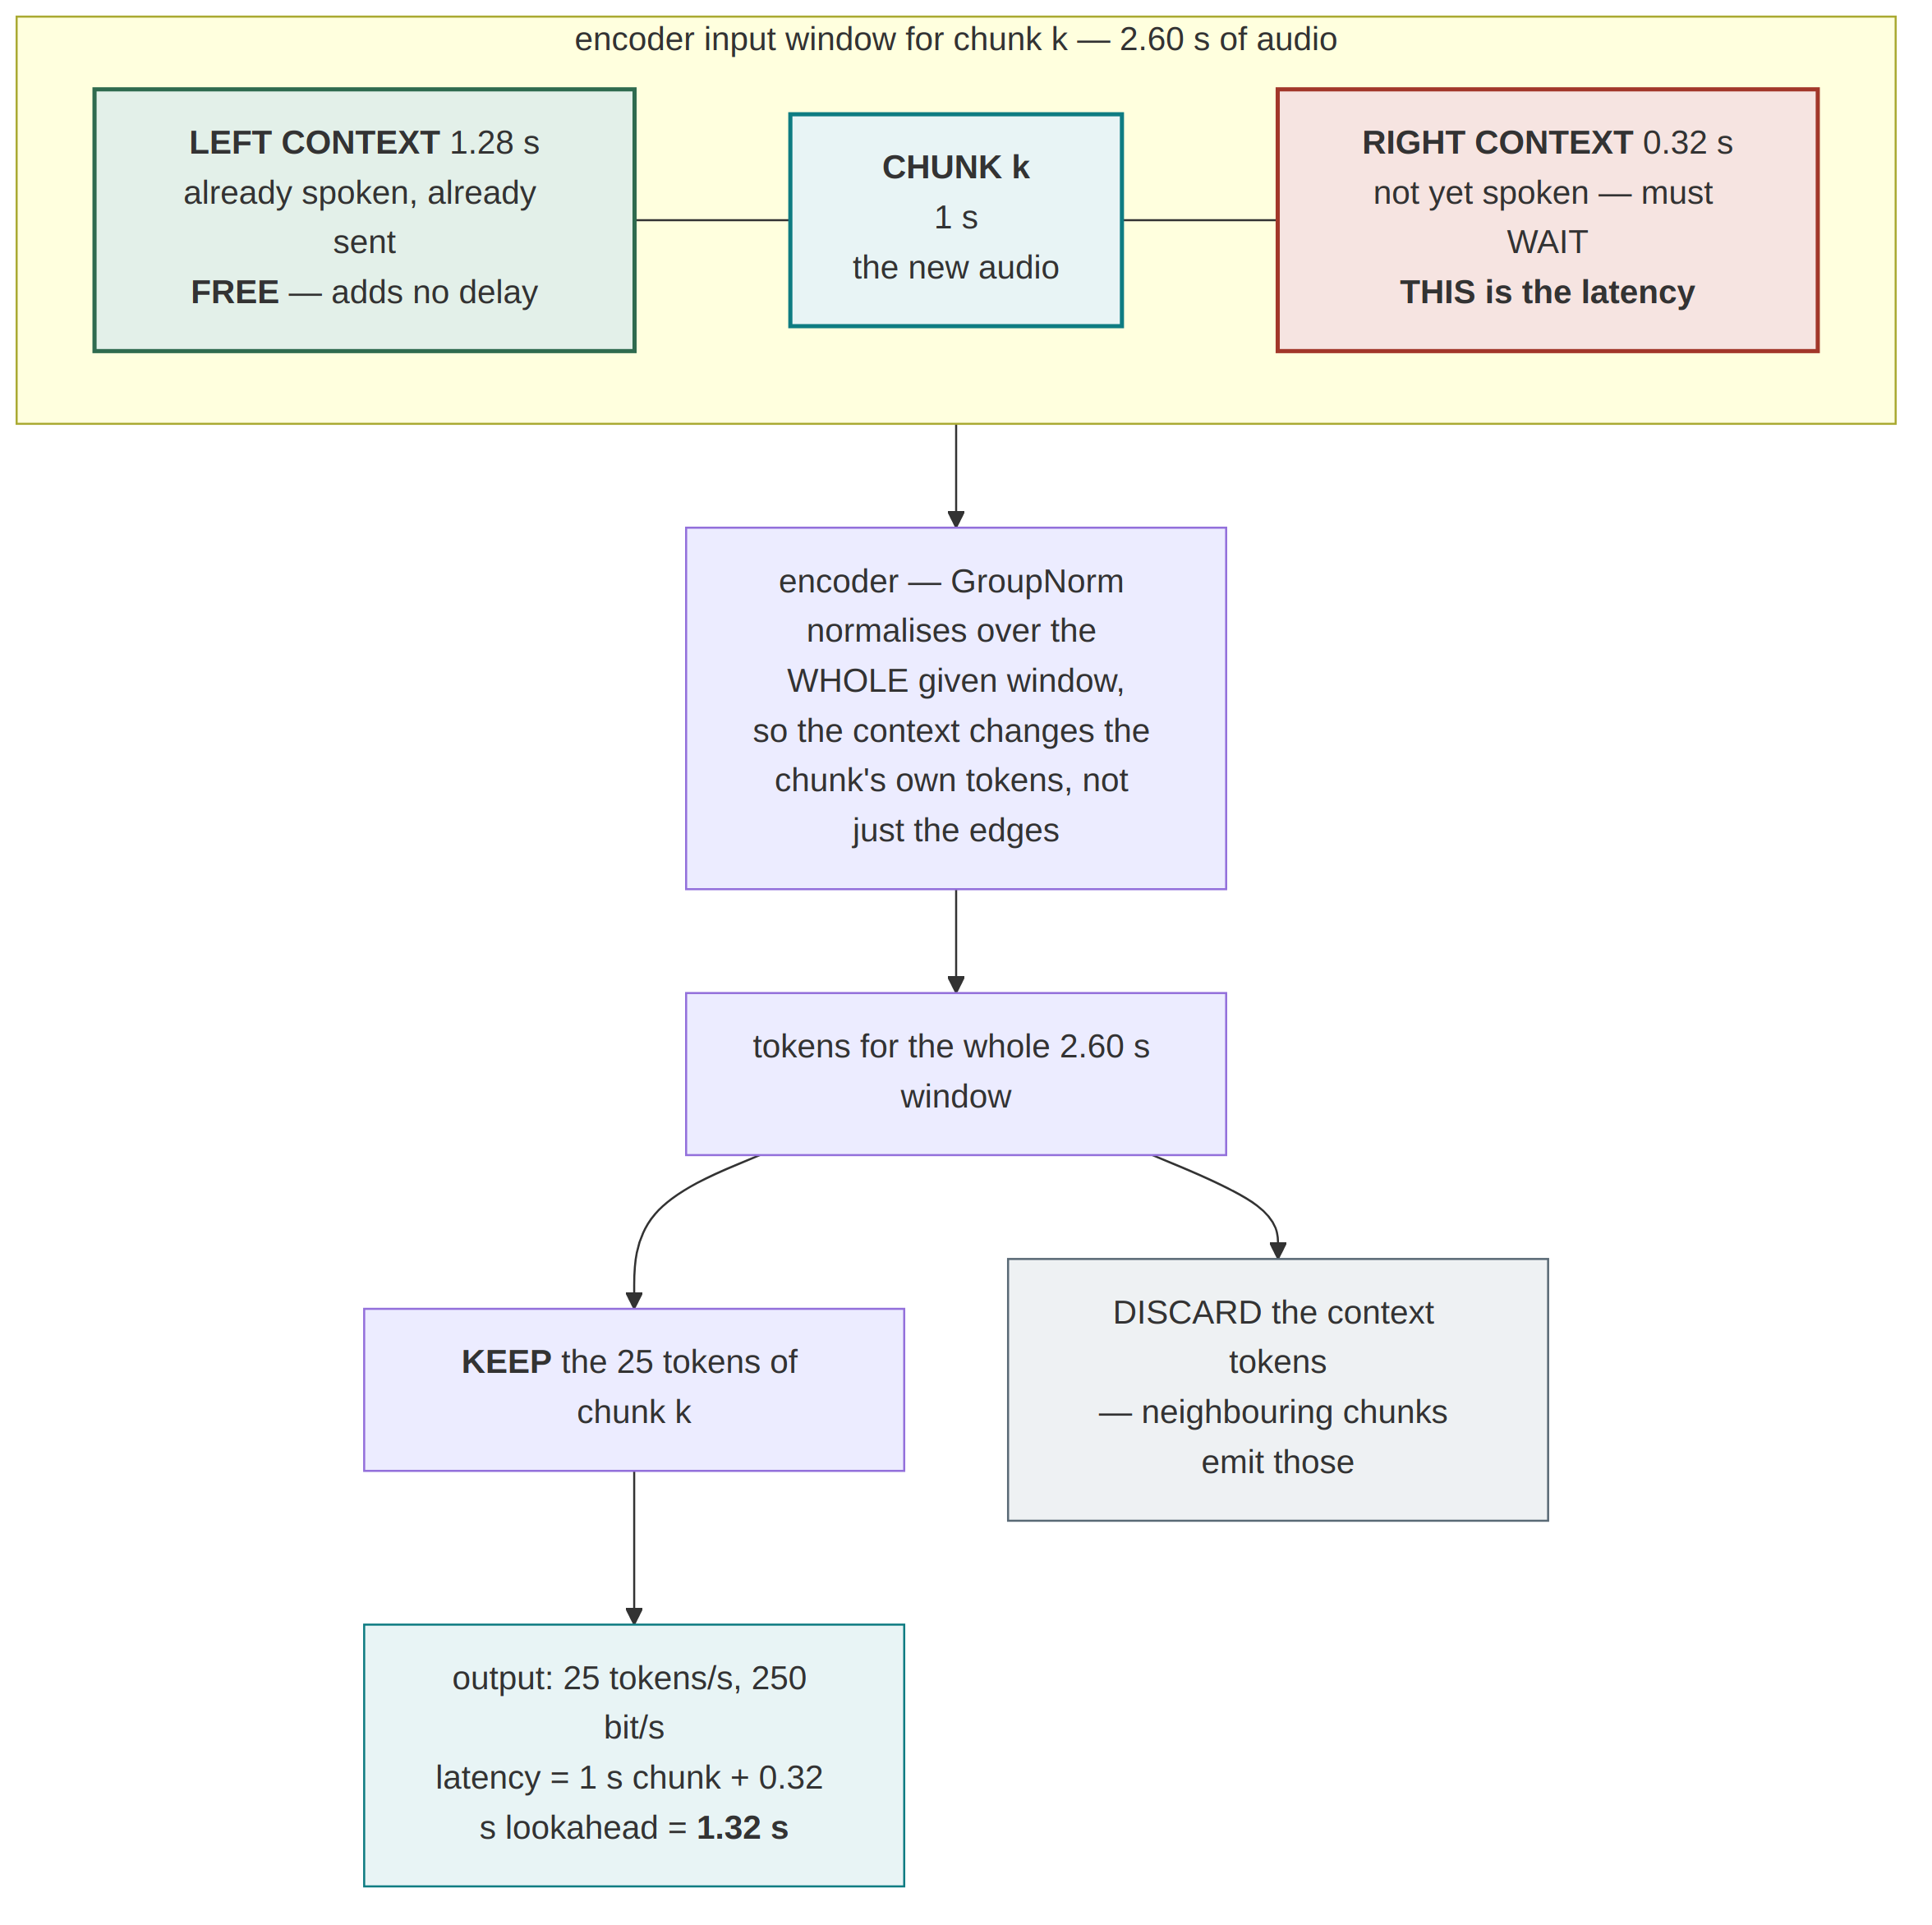
\includegraphics[width=\textwidth,height=0.78\textheight,keepaspectratio]{images/voice_chunk_context.png}
    \caption{One chunk's encoder window.  Only the right context costs
             latency; the left context is audio already in hand.  Because
             the group norm covers the whole window
             (\S\ref{sec:voice_stream}), the context changes the chunk's
             own tokens rather than merely repairing its edges.}
    \label{fig:voice_chunk_context}
\end{figure}

\begin{table}[H]
    \centering
    \caption{Chunk and context against latency, measured on two minutes
             of Russian narration.  Chunk length is nearly irrelevant;
             the last 0.32\,s of lookahead is a cliff.}
    \label{tab:voice_latency}
    \small
    \begin{tabular}{@{}lllrr@{}}
    \toprule
    \textbf{Chunk} & \textbf{Left ctx} & \textbf{Right ctx} &
    \textbf{Latency} & \textbf{mel dB} \\
    \midrule
    6\,s & 1.28\,s & 1.28\,s & 7.28\,s &  7.20 \\
    2\,s & 1.28\,s & 1.28\,s & 3.28\,s &  7.29 \\
    2\,s & 1.28\,s & 0.88\,s & 2.88\,s &  7.33 \\
    2\,s & 1.28\,s & 0.32\,s & 2.32\,s &  7.33 \\
    \textbf{1\,s} & \textbf{1.28\,s} & \textbf{0.32\,s} &
        \textbf{1.32\,s} & \textbf{7.40} \\
    2\,s & 1.28\,s & \textbf{0.00\,s} & 2.00\,s & \textbf{16.76} \\
    \bottomrule
    \end{tabular}
\end{table}

Going from 6\,s chunks to 1\,s costs 0.20\,dB.  Removing the final
0.32\,s of lookahead costs \textbf{9.4\,dB} and the decode collapses.
Quality never depended on chunk length --- only on having \emph{some}
right context --- so the latency was reducible almost for free, and a
listener could not distinguish the 1\,s and 6\,s outputs at all.  The
settled configuration is \textbf{1\,s chunks, 1.28\,s of left context
and 0.32\,s of lookahead}, for 1.32\,s of algorithmic latency, flat
memory, and no change to the model, the bitstream or the protocol.

Chunking costs compute in overlap: each 1\,s chunk re-encodes 1.6\,s of
context around it, and encoding falls from $33\times$ real time at 6\,s
chunks to $17\times$ at 1\,s.  Decoding is unaffected at $5\times$ and is
now the slower half --- the figure a receiver must keep ahead of.

\subsection{Putting It on the Air: the Mode as Built}
\label{sec:voice_onair}

The measurements above are all host-side.  What follows is the codec
actually running between the two boards: a browser front end
(\texttt{host/webvoice/}) that drives one board as transmitter and the
other as receiver, holds a push-to-talk button, and writes what the far
station decodes to a \texttt{.wav}.  It works, and how it got there is
more instructive than the fact that it does: one firmware policy that
was right for files and wrong for speech, a receiver that had to learn
to decode as it listened, a decode profile that grew a cost axis, and a
codec that needed a name on the wire.  The group loss that the same
campaign kept reporting has a subsection of its own
(\S\ref{sec:voice_loss}).

\subsubsection{From the design to the air}
\label{sec:voice_design}

Figure~\ref{fig:voice_mode_design} is the design the evaluation
supported before anything was built, and it is kept here as drawn
because the distance between it and what runs is the content of this
subsection.  It committed to every component being host-side, with
\texttt{cport/} and the wire format unchanged.  Three of its four
commitments survived; the transport, the latency policy and the
``no firmware change'' did not.

\begin{figure}[htbp]
    \centering
    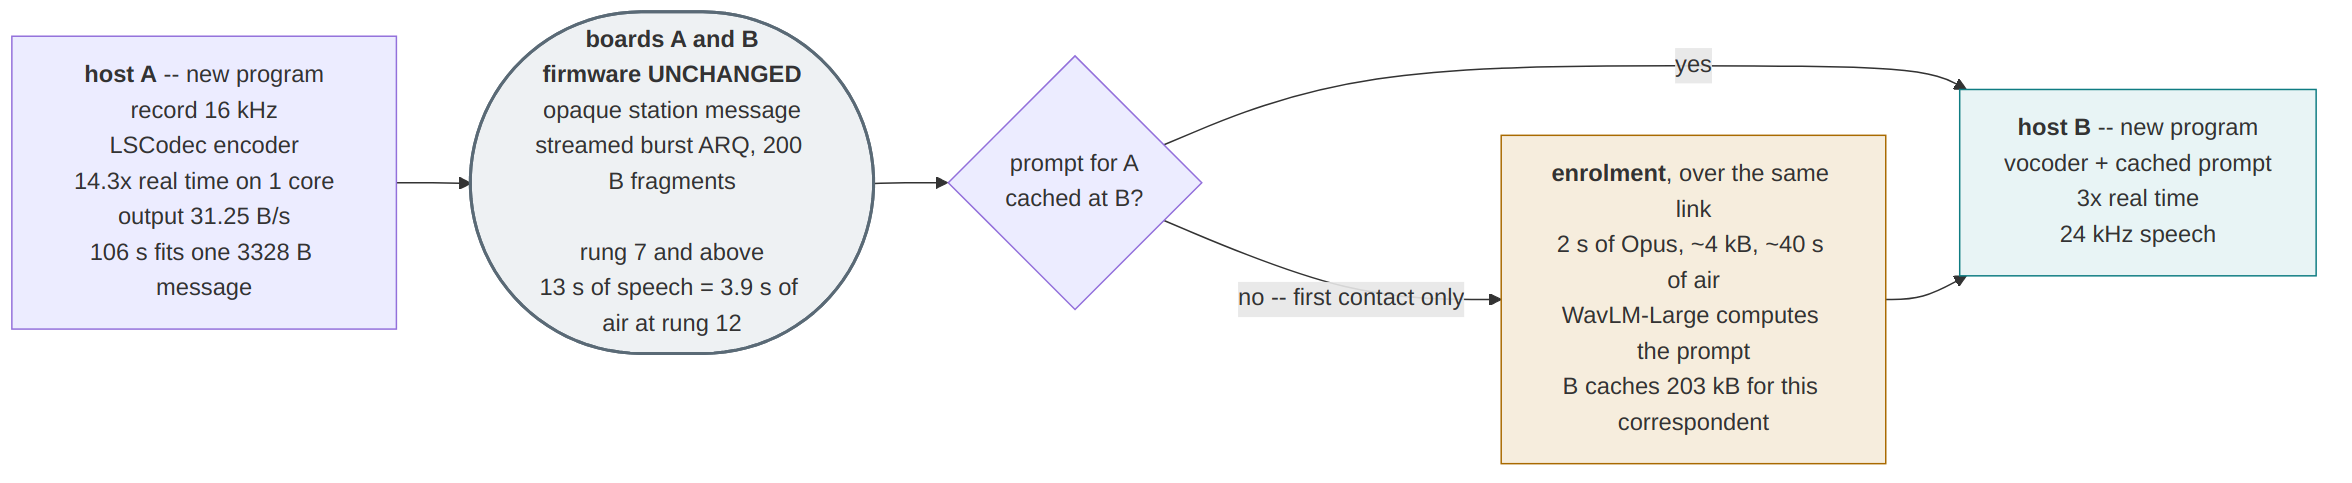
\includegraphics[width=\textwidth]{images/voice_mode_design.png}
    \caption{The voice mode as first proposed, before it was built.
             The tokens were to ride the streaming burst machinery as
             an opaque payload; as built they ride broadcast with a
             named payload type, and the firmware gained a real-time
             keying flag (below).}
    \label{fig:voice_mode_design}
\end{figure}

The design committed to four things the measurements decided.
Enrolment is \emph{audio}, not features, and happens once per
correspondent (\S\ref{sec:voice_promptsize}); the cached prompt is
int8 per-channel, 105\,kB; the speaker's identity travels in the
prompt, never in the payload, so a station that has not enrolled a peer
cannot render that peer's voice at all --- a feature for the
identification question and a constraint on the protocol.  The fourth
--- the mode is real time from rung~7 upward and store-and-forward
below --- was half right: real time is what was built, and the
store-and-forward half was rejected once a receiver that decodes as it
listens existed (\S\ref{sec:voice_decode}).  In the build the
enrolment exchange itself is not yet on the air: the receiver derives
the prompt from the first two seconds of the session it decodes, which
is the transmitter's own voice, and a stored per-correspondent prompt
is where the design's enrolment message would land.

Two paths lead off this design, and they differ in what they cost the
wire.  Fine-tuning the \textbf{vocoder} on in-domain or Russian speech
changes no bitstream: a peer with stock weights still decodes, a peer
with tuned weights decodes better, and there is no capability bit.
Adopting a \textbf{global speaker token} in place of the prompt would
collapse enrolment to about ten bytes, but requires retraining the
prompt path and therefore matching models at both ends --- and, per
LSCodec's own comparison, would trade away some of the speaker
similarity that made this codec attractive: LSCodec reaches 0.853 SECS
at 0.25\,kbps where TiCodec reaches 0.714 at 0.75\,kbps, precisely
because it spends no bits on identity.

\subsubsection{Transport, and the bit alignment that makes a lost group a gap}
\label{sec:voice_transport}

Transport is \textbf{broadcast} (\texttt{PKT\_TYP\_BCAST}, ptype~15 at first, \texttt{BC\_PT\_LSCODEC\_25} once the codec had a name, below),
not the ARQ path.  For speech a late repeat is worth less than a gap:
the same 20\,s utterance costs 2.0--5.2\,s per message through the
acknowledged path against 0.9\,s broadcast, and a retransmission that
arrives after the listener has moved on is pure harm.  Nothing is
acknowledged and nothing is repeated.

The token packer emits ten bits each and zero-pads to a byte boundary,
so 50 tokens is 500 bits in 63 bytes --- four pad bits.  Independently
packed groups are then concatenated by the receiver, which has no
framing inside the stream and unpacks the whole thing as one bit
sequence.  Every group after the first is therefore shifted by four
bits, then eight, then twelve.  The symptom is diagnostic in hindsight:
the first second of every transmission decoded perfectly and everything
after it was noise, which reads like a channel that collapses and is
arithmetic.  The fix is to emit only multiples of \textbf{four} tokens
--- 40 bits is exactly 5 bytes --- and carry the remainder into the
next group.  Verified 300/300 tokens bit-exact end to end.

\subsubsection{The real-time flag: the latency was the group rule, not the codec}
\S\ref{sec:voice_latency} settles the codec at 1.32\,s.  The radio then
added four more, and none of it was DSP\@.  The firmware keys only
\emph{full} groups while chunks are still arriving, which is correct
for a file --- a starved tail group would go out without EOS, and the
true last frame must carry it --- but a group is
$\texttt{BC\_GROUP}\times(\texttt{BC\_FRAME}-2) = 96$ bytes, and at
250\,bit/s that is 3.1\,s of talking that must accumulate before the
first carrier goes up.

This is the first place \texttt{cport/} changed.  A real-time flag
(ptype bit 5, \texttt{BC\_RT}) keys what is queued instead of waiting.
It has three parts and the middle one is the trap: the group must
shrink to a \emph{power of two} matching the frames actually keyed,
because the SYNC descriptor carries $\log_2(\text{group})$ and a
receiver told to expect four blocks when three were sent walks into a
block that never comes and goes deaf for a block time --- the same
failure that once made streamed bursts loop.  The flag is opt-in and
off for every other broadcast, since a smaller group is a preamble per
fewer frames and trades air time for latency.

A second, duller second and a half was the machine learning framework:
the first encode cost 826\,ms against 47\,ms for every one after, all of
it lazy allocation and kernel selection landing on the first
transmission.  Warming the graphs at startup moves it where nobody is
listening.  Together: first audio at the far station about
\textbf{3.6\,s} after the talker starts, against roughly 6\,s before.

\subsubsection{The receiver has to decode as it listens}
\label{sec:voice_decode}
An algorithmic latency of 1.32\,s is a property of the codec, not of a
system, and the first working receiver threw all of it away: it
accumulated the whole transmission and vocoded once at end-of-stream,
so the listener heard the first word only after the last one had been
spoken.  On a 200\,s transmission that is $\sim$202\,s of latency for
word one --- a store-and-forward voicemail wearing a real-time
codec's clothes.

Decoding a chunk at a time as the tokens land is not free, because the
vocoder normalises over time exactly as the encoder does
(\S\ref{sec:voice_stream}): a chunk decoded in isolation drifts from
what the one-shot decode would have produced.  Left context repairs it,
and --- this is the part that makes streaming decode viable at all ---
left context costs \emph{no latency}, because those tokens have already
arrived and already been played.  Lookahead would cost latency, and the
decoder uses none.

\begin{table}[H]
    \centering
    \caption{Chunked vocoding against the one-shot decode of the same
             received bytes, 1\,s decode steps.  Log-spectral $L_1$; a
             waveform metric cannot measure this at all (below).}
    \label{tab:voice_decctx}
    \small
    \begin{tabular}{@{}lrl@{}}
    \toprule
    \textbf{Left context} & \textbf{log-spec $L_1$} & \\
    \midrule
    0.0\,s & 0.3169 & chunks decoded in isolation \\
    1.0\,s & 0.2341 & \\
    \textbf{2.0\,s} & \textbf{0.2240} & the knee, and what ships \\
    4.0\,s & 0.2174 & twice the context for 3\,\% \\
    \bottomrule
    \end{tabular}
\end{table}

Measured end to end on the two-board stand, the assembled output
measures 0.2044 against a one-shot decode of the identical received
bytes, at identical length, slightly better than the offline sweep
predicted; a 200\,s transmission delivers 325 frames, zero lost,
byte-exact, with end-to-end lag flat at 0.000\,s per second of
speech.  The first-audio figures moved twice more after this
paragraph was first written and are reported with the profiles below,
where they belong.

One methodological note, because it cost a measurement.  The first
version of this sweep used waveform RMS error and reported $\approx
1.0$ at every context length --- which reads as ``chunking destroys the
audio'' and is meaningless.  A vocoder is \emph{generative}: two
decodes of the same tokens differ in phase and agree perceptually, so a
waveform metric is uncorrelated with quality by construction.  The
encoder study in \S\ref{sec:voice_stream} already used a spectral
metric for this reason; the right move was to read it first.

\subsubsection{Profiles: the decode latency becomes a knob, and grows a cost axis}
The left context above is fixed at 2\,s and free; two other quantities
are not, and together they define a decode \emph{profile}: the
\textbf{chunk} (how much speech each step emits --- the listener waits
for the first one to fill) and the \textbf{lookahead} (tokens beyond
the chunk fed to the vocoder and discarded --- each second of it is a
second of added latency).  Both improve quality.  What forced the
profile table through three revisions is that they also cost
\emph{compute}, and a step must finish inside its own chunk's duration
or the decoder falls behind speech without bound.

\begin{table}[H]
    \centering
    \caption{Chunk and lookahead against quality and cost.  $L_1$ is
             log-spectral distance to the one-shot decode of the same
             received bytes; duty is measured step time over the chunk
             duration, on both devices the host supports.}
    \label{tab:voice_profiles}
    \small
    \begin{tabular}{@{}llrrrrl@{}}
    \toprule
    \textbf{Chunk} & \textbf{Ahead} & \textbf{Latency} &
    \textbf{$L_1$} & \textbf{GPU} & \textbf{CPU} & \\
    \midrule
    1\,s & 0\,s & 1\,s & 0.2240 & 15\,\% &  77\,\% & \texttt{live} \\
    1\,s & 1\,s & 2\,s & 0.1236 & 19\,\% & \textbf{100\,\%} &
        \texttt{balanced} (GPU) \\
    2\,s & 1\,s & 3\,s & 0.1113 & 12\,\% &  63\,\% &
        \texttt{balanced} (CPU) \\
    2\,s & 2\,s & 4\,s & 0.1108 & 15\,\% &  83\,\% & dominated \\
    3\,s & 2\,s & 5\,s & 0.0941 & 11\,\% &  60\,\% & \texttt{quality} \\
    \bottomrule
    \end{tabular}
\end{table}

Three lessons are in this table, each paid for.  First, the 1\,s/1\,s
shape was shipped as \texttt{balanced} after measuring only its
quality; at exactly 100\,\% CPU duty it could not keep up, and the
processor it saturated starved the browser's main-thread capture into
delivering silence --- the cost column exists because the quality
column alone chose an infeasible configuration.  Second, on the CPU a
\emph{bigger chunk is both better and cheaper}: the fixed left context
is paid once per step, so amortising it over more output lowers the
duty and removes seams together --- the best row is also the cheapest,
and varying lookahead alone was the wrong knob.  Third, the entire
constraint was an artefact: nothing had ever moved the models off the
CPU.  On the GPU a decode step falls from 830\,ms to 148\,ms, every
shape in the table is idle-cheap, and the choice collapses to latency
against quality --- which is what a profile should have been all
along.  The operator picks \texttt{live}, \texttt{balanced} or
\texttt{quality} per transmission; the page's option list is generated
from the server's own table so the interface cannot drift from what
was measured.

Measured on the air, 40\,s per profile, all byte-exact with zero loss:
first audio \textbf{3.6\,s} (\texttt{live}), \textbf{4.8\,s}
(\texttt{balanced}), \textbf{8.5\,s} (\texttt{quality}) after the
talker starts, with end-to-end lag drift of $-0.005$, $-0.014$ and
$-0.005$\,s per second of speech --- every profile holding steady where
the mis-costed one drifted without bound.

\subsubsection{The codec gets a name on the wire}
While one codec was the only voice on the air it rode on the OPAQUE
payload type and a receiver could only guess from the byte rate.  Two
small protocol changes make a second codec possible before it exists.
The broadcast SYNC descriptor's payload-type registry --- which had
reserved Codec2 entries from the start --- gains
\texttt{BC\_PT\_LSCODEC\_25}; the ptype is a label rather than a
demultiplexer, so a receiver that does not know the codec still stores
the bytes exactly as before.  And the capability record
(\S\ref{sec:cport_caps}) gains a codec bitmap: which voice codecs a
station can \emph{decode}, so a sender picks one the far end can play.
The record grew from 10 to 11 bytes and the version deliberately did
not move --- an older record parses with the new field reading
``never said'', an older peer takes the prefix it knows, and both
directions keep working, which is the one property a capability
mechanism cannot trade away.  The codec itself lives in the HOST, not
the board --- the board moves bytes --- so the host declares its
codecs over USB (a config key) and reads the peer's declaration back
from the status frame, both under the same grow-only contract the
temperature and rung fields established.  Verified on the stand: the
handshake completes with the codec bit crossing the air and arriving
at the far host.

\subsection{Group Loss on a Clean Wire: Three Answers}
\label{sec:voice_loss}

The transmissions kept reporting losses --- 7.7\,\%, 11.8\,\%,
14.4\,\% of bytes --- on a cross-wired pair at rung~12 carrying
250\,bit/s.  On a channel with tens of decibels of margin and a duty
cycle this low that looks impossible, and chasing it produced two
wrong answers before the right one.  All three are reported, because
how each wrong one survived its own round of measurement is the more
useful part --- and because the right one ended in the firmware, not
in an explanation.

A lost unit is always the same shape: \textbf{one group, lost whole}
--- 30 or 35 bytes depending on how the group was sized, about a
second of speech.  Three independent measurements agree.  The recording
comes back short by exactly that much; the byte streams differ by
exactly that much; and the sent/received dump names the offset:

\begin{quote}\ttfamily\small
sent 660 B, received 630 B, missing 30 B\\
streams agree for the first 310 B\\
$\Rightarrow$ 30 B missing at offset 310\\
\hphantom{$\Rightarrow$} resumes at sent-offset 340; tail after that matches
\end{quote}

\noindent
The receiver never acquires that group's preamble.  That is why nothing
anywhere logged it: no walk is entered, so no failed-block event fires,
and the loss is discovered only from the sequence gap in the \emph{next}
SYNC\@.  A silent failure of this shape is what the sequence field
exists for.

Three candidate causes were eliminated by counter rather than by
argument, which is the only way to make progress on a fault that logs
nothing.  The receiving board's capture-FIFO overrun counter stayed at
zero across every losing run --- it was not dropping samples.  Its
\texttt{bc\_rx\_lost} beacon counter, which only the failed-block path
increments, also stayed at zero --- the frames were never \emph{heard},
not mis-decoded.  And the mid-stream broadcast statistics exchange,
which does make the receiver key a frame, showed no correlation.

Two genuine host defects were found on the way and are worth having
regardless of what caused the loss.  The first is a race: the web
server is threaded and the browser posted audio fire-and-forget, so the
encoder and the broadcast sender ran on several threads at once ---
\textbf{27 collisions in a single 20\,s transmission}, counted.  The
damaging one is the broadcast-open flag, read \emph{before} the USB
write and assigned \emph{after} it, so two threads both see it clear and
both send a non-continuation command; the firmware treats the second as
a new broadcast, closing the one on the air and resetting the sequence.
The second is the warm-up, which was declared complete the moment the
far station \emph{decoded} the message --- while the acknowledgement it
owed was still to be keyed, and the link is half duplex.  Both are
fixed.  Neither was the cause.

\subsubsection{The first answer, and how it survived its measurement}
The warm-up defect predicts losses at the \emph{head} of a stream, and
the first evidence agreed: 5 losses in 23 transmissions without the fix
against 0 in 16 with it, Fisher $p = 0.066$, and three of four
recoverable loss positions near the start.  That is a plausible-looking
result, and it was wrong twice over.  The loss positions came from
correlating audio envelopes, which is too blunt to locate a
one-second gap in a re-synthesised waveform; and the two arms were
measured an hour apart, so anything that drifted was attributed to the
fix.

Repeating it properly settles it.  Twelve \emph{interleaved} pairs ---
the arms alternating within each pair, so drift cannot favour either
--- give 1 loss in 12 with the fix against 2 in 12 without,
$p = 1.000$.  There is no effect.  The earlier sixteen clean
transmissions were chance, and the interleaved design is what exposes
that.  By then the byte dumps were in place, and they close the
argument outright: the gaps sit at 0.96\,s, 6.88\,s, 9.92\,s, 10.88\,s
and 17.92\,s into their streams --- \emph{uniformly spread}, with one
transmission losing two.  A warm-up that finished twenty seconds
earlier cannot miss a group at 10.88\,s.

\subsubsection{The second answer, and how it fell}
The natural conclusion at this point --- and the one a draft of this
section briefly drew --- was that 0.76\,\% is simply the acquisition
statistics of non-acknowledged broadcast: \S\ref{sec:cport_bcast}
records 38 of 39 groups across an earlier campaign at rung~4, a
2.6\,\% loss rate, and the voice path was running three times better
than that.  Acquisition is a threshold decision, a high
signal-to-noise ratio makes a miss unlikely rather than impossible,
and nothing in a broadcast retries.  Plausible, self-consistent, and
wrong --- the instinct that a clean channel should lose nothing was
right all the way down.

What broke this one was refusing to accept ``statistics'' without a
reproduction.  A soak bench (\texttt{make bcsoak}) drives the
firmware's own group build-and-walk through the streaming receiver at
the voice shape --- two-frame groups, random payload, random gaps,
random sample-phase lead, thousands of groups --- and the loss
reproduced \emph{on the host}, with no noise, no boards and no air:
28 of 720 frames, deterministic per seed, every missed group starting
in the same $\sim$8-sample window of alignment mod 256.  A rate that
depends on sample phase is not statistics.

\subsubsection{The actual defect}
Traced on a failing seed: a tone field \emph{entering} the detection
window can produce one isolated above-threshold evaluation --- metric
$\sim$$5\times10^{7}$ against $\sim$$10^{11}$ for the aligned peak, at
a coarse-frequency shift of $-5$ bins --- whose above-threshold region
dies immediately.  The detector's region-argmax rule committed it,
anchoring two blocks before the real preamble.  The header then fails,
and the recovery rearm does exactly what its comment has promised all
along --- ``the true preamble, still in the ring, can be re-acquired''
--- except that nothing ever looked: the search only evaluated the
\emph{newest} block, so every window between the failed anchor and the
present was skipped, and the failed ZC and header attempts had
meanwhile consumed the true peak's samples.  Three garbage attempts
walk straight over the group.  The comment described a recovery the
machinery never performed.

Two fixes were built, and the difference between them is the useful
part.  The first made the machinery match the comment: rewind the
search after a failure and recompute block summaries from the raw
ring.  It passed every host suite, the robustness gate and an 1800-group
soak --- and melted both boards within minutes of flashing:
at EXTREME, failed acquisitions on plain noise are routine, each one
re-scanned its whole excursion, and the capture FIFO never recovered
(4.8 million dropped samples on the receiving board, which decoded
nothing at all).  No host bench models EXTREME-scale CPU under a
failure loop, which is exactly why it survived validation.  The second
fix is three lines and does strictly \emph{less} work than the
original code: the fast region-end commit now requires the metric to
be \emph{strong} ($\geq 64\times$ the threshold; real peaks measure
$10^{4}$--$10^{6}\times$), and a weak argmax takes the
argmax-stability path the code already had --- during which the true
peak's evaluations arrive and replace it.  The garbage is never
committed at all.  Prefer not committing garbage over recovering from
having committed it.

Validation, in the order it should have happened the first time: the
soak falls to 0 lost in 1800 groups; a gate-on/gate-off A/B at the
EXTREME sensitivity knee decodes \emph{identically} at every
signal-to-noise point with zero false alarms in both arms; and on the
reflashed boards, \textbf{24 of 24 live voice transmissions
($\sim$900 frames) crossed with zero loss} --- with the warm-up settle
deliberately disabled in half of them, which is what being the actual
cause looks like.  Against the pre-fix 21.7\,\% per-transmission rate,
24 clean runs is $p = 0.003$.  Whether the earlier rung-4 campaign's
2.6\,\% shares this cause cannot be settled retroactively, but the
soak now guards the code path either way.

The methodological lesson is the expensive one and worth stating
plainly.  A fault that logs nothing invites the investigator to supply
the missing narrative, and this one collected \emph{three} narratives
--- a timing fix confirmed by two rounds of measurement, then ``by
design'' backed by a plausible reference rate --- before the real
defect surfaced.  Each fell to the same move: make the evidence harder
to flatter.  Interleave the arms so drift cannot masquerade as an
effect; keep the raw artefact (the byte streams) rather than a
statistic derived from it; and refuse ``statistics'' as an explanation
until the statistic survives a reproduction attempt.  All three were
cheap, and none was done first.  The one that found the bug --- soak
the exact code path at scale on the host --- also produced the second
regression, because host validation cannot see embedded CPU: the
firmware that shipped was proven on the bench \emph{and} the stand,
and both proofs were necessary.

\subsubsection{Why a lost group is survivable at all}
The byte-alignment fix has a consequence worth stating separately,
because it is the property that makes non-acknowledged voice viable.
Once every group is a whole number of bytes carrying a whole number of
tokens, a group that never arrives is a \emph{gap} --- the decoder
resumes in step on the next one.  Before the fix, the same lost group
desynchronised everything after it.  This is why a transmission
measured at 7.7\,\% loss was still clearly intelligible: the listener
hears a missing syllable, not a collapse.  It is also the argument for
broadcast over ARQ at this bitrate, made concrete: the failure mode of
dropping a group is bounded, local, and about a second long.

This property remains load-bearing even now that the 0.76\,\% turned
out to be a fixable defect: over a real fading channel, groups WILL be
lost, no acknowledgement will recover them, and byte-aligned groups
are what convert each loss into a missing syllable rather than a
desynchronised remainder.  The clean-wire campaign proved the
tolerance works; the fix means it is no longer being spent on the
receiver's own commit rule.

\subsection{Where This Leaves a Voice Mode}
\label{sec:voice_status}

The bitrate fits, the compute fits, and the transport needed less
change than a new mode usually does: the tokens are opaque bytes on the
broadcast path the firmware already had, with a payload type to name
them and a capability bit to say who can play them.  A voice mode is a
host program, like KISS and the IP tunnel, and \S\ref{sec:voice_onair}
is that program working between two boards.
It is also not store-and-forward: \S\ref{sec:voice_latency} settles
the codec at 1.32\,s of algorithmic latency with flat memory, an order
of magnitude below the link's own turnaround --- provided the receiver
decodes as it listens rather than at end-of-stream
(\S\ref{sec:voice_onair}), which is a property of the implementation
and not of the codec, and which the first working receiver got wrong.

The firmware changes are worth recording, because the design of
\S\ref{sec:voice_design} predicted none and was wrong for an
instructive reason.  Every host-side measurement was of the
\emph{codec}, and the codec was never the problem: the radio's own
rule that a broadcast keys only full groups is correct for a file and
is, for speech, three seconds of latency that no amount of chunk tuning
can reach.  A knob that a caller can decline (\texttt{BC\_RT}) was
the right shape, because the rule it waives is still right for
everything else.  The other two changes --- a payload type and a codec
bitmap in the capability record --- were protocol hygiene the first
codec could have done without and the second cannot; and the detector's
commit gate (\S\ref{sec:voice_loss}) was not a voice change at all but
a receiver defect that only a mode without retransmission could have
exposed.  The
general lesson is the one this chapter keeps arriving at: a policy that
is correct for the traffic it was written for becomes a defect when a
new class of traffic arrives, and the fix is to make it a choice rather
than to change it.

Two defects are characterised rather than fixed.  The English accent of
\S\ref{sec:voice_russian} is the cheaper one, and sits in the
fine-tunable half.  The other is unresolved: the failure \emph{rate} on
real shack audio.
Three destroyed utterances in sixteen was measured on read speech one
corpus away from training; the Russian measurements suggest the
degradation is graceful there ($+1.58$\,dB over five minutes of
narration, and one phone-grade sentence intelligible), but neither is
a catastrophic-failure \emph{rate} on shack audio.  That number, and
not the bitrate, decides the question ---
because a transmission that arrives as fluent nonsense with every
protocol counter healthy is worse than one that fails.

Fine-tuning is the obvious remedy and splits usefully.  The
vocoder (31.3\,M parameters) can be fine-tuned without touching the
codebook, which means \textbf{the bitstream does not change}: a peer
running stock weights still decodes the transmission, a peer with the
tuned weights decodes it better, and no capability bit or protocol
revision is involved.  Retraining the encoder and quantiser would
change what the tokens mean and \emph{is} a protocol change, requiring
both ends to match.  Neither fixes the identity property, which is the
architecture working as designed.
